\documentclass[a4paper,10pt]{article}
\usepackage[pdftex]{graphicx}
\usepackage{polski}
\usepackage[utf8]{inputenc}
\usepackage{textcomp}
\usepackage{pifont}
\usepackage{color}
\usepackage{listings}

% opcje listingów
\definecolor{darkgray}{rgb}{0.95,0.95,0.95}
\lstset{language=c++}
\lstset{backgroundcolor=\color{darkgray}}

\title{\textbf{Biologia obliczeniowa}}
\author{\textbf{Mateusz Cicheński} [84780, I1]\\ \textbf{Tomasz Żurkowski} [84915, I1]}
\date{24 kwietnia 2010 r.}

\begin{document}
 
\maketitle

\tableofcontents

\newpage

\section{Wprowadzenie do zagadnienia}

Problem sekwencjonowania łańcuchów DNA jest w ogólności problemem silnie NP-trudnym. W problemie tym mamy dany zbiór {\bf S} słów (oligonukleotydów) o jednakowej długości {\bf l} nad alfabetem {\bf \{A, C, G, T\}}. Ponadto mamy podaną długość sekwencji oryginalnej {\bf n}. Celem sekwencjonowania jest odtworzenie oryginalnego łańcucha DNA, który został poddany hybrydyzacji, na podstawie powyżej zdefiniowanych danych wejściowych.
Dla ułatwienia dalszego opisu wprowadźmy kilka terminów: 
%TODO więcej terminów?
\begin{description}
  \item[Odległość między oligonukleotydami] definiuje się między każdą parą słów jako najmniejsze przesunięcie jednego oligonukletydu względem drugiego, które umożliwi połączenie ich w jeden łańcuch. Dla przykładu słowo $ACGTA$ znajduje się w odległości 2 względem słowa $ACACG$ (relacja w drugą stronę - słowo $ACACG$ znajduje się w odległości 4 względem słowa $ACGTA$).
%TODO
%   A C A C G
%       | | |
%       A C G T A
% Odleglłość między olignukleotydem ACACG a ACGTA

  \item[Spektrum] %TODO
  \item[Sekwencja DNA] %TODO
  \item[Błąd negatywny]
  \item[Błąd pozytywny] 
  \item[Graf DNA]
\end{description}
W zaproponowanych przez nas podejściach będziemy wykorzystywać teorię grafów w celu szybkiego łączenia oligonukleotydów oddalonych od siebie o jak najmniejszą wartość.

W analizie problemu można wyróżnić cztery szczególne przypadki - idealny, z błędami negatywnymi, z błędami pozytywnymi, z obydwoma typami błędów.
Przypadek idealny to taki, gdzie na mikromacierzy dopasowały się wszystkie słowa występujące w sekwencji.
Mówimy, że dane odwzorowanie łańcucha DNA na mikromacierzy zawiera błędy negatywne, jeśli z jakiegoś powodu niektóre słowa nie zostały dopasowane do macierzy. Otrzymujemy więc niepełne spektrum sekwencji.
Błędami pozytywnymi określamy nadmiar informacji, tzn. na mikromacierzy zostały dopasowane słowa, które nie występują w sekwencji oryginalnej. Mamy więc zbiór słów które są nadzbiorem zbioru słów wchodzących w skład oryginalnej sekwencji.

\section{Generowanie losowych instancji SBH}

%TODO Tutaj o generowaniu instancji ...

\section{SBH z błędami pozytywnymi}
Jak już wcześniej mówiliśmy, sekwencjonowanie łańcucha DNA z błędami pozytywnymi charakteryzuje się nadmiarową ilością słów otrzymanych w spektrum. Mamy więc pewność, że pośród tych słów znajdzie się dokładnie $n-l+1$ z których będziemy mogli zrekonstruować oryginalną sekwencję.

Wprowadźmy na początku pomocniczy algorytm usuwania cykli z grafu $G$:

Algorytm 1:
\begin{enumerate}
 \item Znajdź silnie spójne składowe grafu $G$
 \item Jeśli w grafie nie ma silnie spójnych składowych, zakończ algorytm
 \item Uszereguj je topologicznie, traktując każdą silnie spójną składową jako wierzchołek oraz tworząc łuk z silnie spójnej składowej $SCC1$ do $SCC2$ jeśli jakikolwiek wierzchołek z $SCC1$ łączy się z dowolnym wierzchołkiem z $SCC2$
 \item Dla danej silnie spójnej składowej $SCC$ znajdź należący do niej wierzchołek $k$, który łączy się z pozostałymi silnie spójnymi składowymi lub weź dowolny wierzchołek jeśli nie ma połączeń z innymi silnie spójnymi grafu
 \item Usuń wszystkie połączenia wychodzące z $k$, które łączą się z innymi wierzchołkami wchodzącymi w skład $SCC$
 \item Idź do punktu 1
\end{enumerate}

Złożoność powyższego algorytmu to $O(S + A + S * (S + A))$. Wynika to ze złożoności kolejnych jego kroków:
\begin{itemize}
 \item $O(S + A)$ dla punktu 1, gdzie liczba łuków jest zależna od słów tworzących spektrum i na pewno nie większa niż $S * (S-1) / 2$
 \item $O(S + A)$ dla punktu 3
 \item $O(S)$ dla punktu 4
 \item $O(1)$ dla punktu 5
\end{itemize}

Mając do dyspozycji algorytm usuwania cykli w grafie proponujemy następujący algorytm rozwiązujący problem sekwencjonowania DNA z błędami pozytywnymi:

Algorytm 2:
\begin{enumerate}
 \item Utwórz graf skierowany {\bf G}. Niech zbiór wierzchołków V stanowią słowa tworzące spektrum sekwencji DNA. Dla każdej pary wierzchołków $(i,j)$ dodaj łuk od wierzchołka $i$ do $j$ wtw gdy słowo w wierzchołku $j$ jest oddalone o 1 od słowa w wierzchołku $i$
 \item Usuń cykle w grafie {\bf G} tworząc graf {\bf RES} korzystając z Algorytmu 1.
 \item Uszereguj topologicznie {\bf RES}
 \item Wybierz najdłuższą możliwą ścieżkę w grafie {\bf RES}
\end{enumerate}

Złożoność powyższego algorytmu to suma złożoności jego poszczególnych kroków. Złożoność poszczególnych punktów jest następująca:
\begin{itemize}
 \item $O(S^2)$ dla punktu 1
 \item $O(S + A + S * (S + A))$ dla punkut 2 (zgodnie z opisem algorytmu 1)
 \item $O(S + A)$ dla punktu 3
 \item $O(S + A)$ dla punktu 4
\end{itemize}

\section{SBH general}
W przypadku podejścia ogólnego nie mamy gwarancji, że istnieje ścieżka po łukach o koszcie 1, która utworzy sekwencję odpowiedniej długości. Musimy więc uwzględnić mniej korzystne połączenia o kosztach 2 i wyższych. W związku z tym wykorzystamy algorytm sekwencjonowania z błędami pozytywnymi uogólniając jego działanie. Algorytm po modyfikacji wygląda następująco:

Algorytm 3:
\begin{enumerate}
 \item Wczytaj zbiór wszystkich słów tworzących spektrum do słownika OLIGS
 \item Utwórz graf skierowany {\bf G}. Niech zbiór wierzchołków V stanowią słowa w słowniku OLIGS. Dla każdej pary wierzchołków $(i,j)$ dodaj łuk od wierzchołka $i$ do $j$ o koszcie równym odległości słowa w wierzchołku $j$ względem słowa w wierzchołku $i$
 \item Znajdź najniższy koszt łuku MIN w grafie {\bf G}
 \item Utwórz graf skierowany {\bf G'}, który jest podgrafem grafu {\bf G} i zawiera tylko łuki o koszcie MIN
 \item Usuń cykle w grafie {\bf G'} tworząc graf {\bf RES} korzystając z Algorytmu 1
 \item Uszereguj topologicznie {\bf RES}
 \item Wybierz najdłuższą możliwą ścieżkę {\bf PATH} w grafie {\bf RES}
 \item Usuń ze słownika OLIGS słowa wchodzące w skład ścieżki {\bf PATH}, w zamian dodając słowo utworzone przez połączenie słów zgodnie z kolejnością w ścieżce {\bf PATH}
 \item Jeśli słownik OLIGS zawiera dokładnie jedno słowo, to zakończ, w przeciwnym wypadku idź do punktu 2
\end{enumerate}

Z punktu widzenia złożoności należy zauważyć, że punkt 3 można zrealizować w ramach punktu 2. Zauważmy ponadto, że punkty od 4 do 7 to dokładnie Algorytm 2, z uwzględnieniem łuków o koszcie MIN (zamiast o koszcie 1 jak podano w poprzednim algorytmie). Złożoności pozostałych punktów to:
\begin{itemize}
 \item $O(S^2)$ dla punktu 2
 \item $O(1)$ dla usuwania w punkcie 8, tworzenie słowa jest liniowo od ilości oligonukleotydów, które wchodzą w jego skład
\end{itemize}
W związku z tym ostateczna złożoność algorytmu to $O(S * (S^2 + Algorytm2))$. Przy czym $S$ występuje w najgorszym wypadku, kiedy w grafie wyjściowym będziemy mieć słowa o długości równej liczbie słów instancji i będą istnieć tylko pojedyncze połączenia o kosztach $1, 2, 3, ..., S$.

Ideą algorytmu jest wyszukanie teoretycznie najkorzystniejszych połączeń o koszcie 1 tworzących sekwencje pełne (tj. w ich skład wchodzą tylko istniejące słowa), a jeśli nie uda się utworzyć na ich podstawie sekwencji wyjściowej, to połączenie sekwencji utworzonych w ten sposób uwzględniając brakujące słowa, czyli łącząc łukami o koszcie 2 i wyższymi. 

Przykład:
Dane wejściowe:
$OLIGS = { AGC, GCT, CTG, TGT, GTG, TGA, GAC, ACT }$
$n = 10$

%               ----------------------
%               |                    v
%AGC -> GCT -> CTG -> TGT -> GTG -> TGA -> GAC -> ACT
%               ^      ^      |                    |
%               |      --------                    |
%               ------------------------------------

Powyżej zaprezentowano graf utworzony w kroku 4 dla wartości $MIN=1$. Wcześniejsze kroki są jednoznacznie interpretowalne, a utworzenie pełnego grafu z punktu 2 bardzo zamgliłoby obraz grafu. Usuńmy teraz cykle.
Jak widać w powyższym grafie mamy następujące silnie spójne składowe:
$A$ - {AGC}
$B$ - {GCT}
$C$ - {CTG, TGT, GTG, TGA, GAC, ACT}
Musimy więc rozbić wszystkie silnie spójne składowe usuwając cykle, co umożliwi nam utworzenie nadłuższej możliwej ścieżki od ustalonego punktu.
Uzyskaliśmy tylko jedną silnie spójną składową $C$, która posiada więcej niż jeden wierzchołek, więc ją należy rozbić. Zauważmy, że po uszeregowaniu topologicznie spójnych składowych uzyskamy następujące uporządkowanie: $A->B->C$, a więc bierzemy pierwszy lepszy wierzchołek silnie spójnej składowej C i usuwamy z niego wszystkie łuki. Ponieważ wybieramy dowolny wierzchołek, załóżmy, że jest to wierzchołek $TGT$, usuwamy zatem łuk prowadzący do $GTG$.
Ponownie generujemy silnie spójne składowe grafu:
$A$ - {AGC}
$B$ - {GCT}
$C$ - {CTG, TGA, GAC, ACT}
$D$ - {TGT}
$E$ - {GTG}
Ponieważ znów mamy silnie spójną składową, która ma więcej niż jeden wierzchołek, to z niej będziemy usuwać cykl. Tym razem jednak po uszeregowaniu topologicznie silnie spójnych składowych otrzymujemy zależność $A->B->C->D->E$. Oznacza to, że w silnie spójnej składowej C musimy odnaleźć wierzchołek prowadzący do silnie spójnej składowej $D$. Takim wierzchołkiem jest $CTG$, usuwamy więc z niego wszystkie łuki wychodzące z niego, które prowadzą do innych wierzchołków silnie spójnej składowej $C$. Zostanie usunięty łuk $CTG->TGA$.
W kolejnej iteracji podziału na silnie spójne składowe uzyskamy siedem jedno-elementowych zbiorów, a więc usuwanie cykli możemy zakończyć. Po wykonaniu powyższych operacji graf wygląda następująco:

%AGC -> GCT -> CTG -> TGT    GTG -> TGA -> GAC -> ACT
%               ^      ^      |                    |
%               |      --------                    |
%               ------------------------------------

Po uszeregowaniu topologicznie możemy uzyskać m.in. następującą kolejność wierzchołków:
$AGC, GCT, GTG, TGA, GAC, ACT, CTG, TGT$
Szukamy najdłuższej możliwej ścieżki korzystając z uporządkowania topologicznego:
$GTG, TGA, GAC, ACT, CTG, TGT$
I tworzymy nowe słowo sklejając poszczególne elementy ze sobą w sekwencję $GTGACTGT$.
Usuwamy wierzchołki, z których utworzyliśmy powyższą sekwencją. Dodajemy otrzymaną sekwencję do grafu, który obecnie wygląda następująco:

AGC -> GCT         GTGACTGT

Uwzględnione są tylko łuki o koszcie $MIN=1$ (czyli niejako uzyskaliśmy las grafów). Ponieważ nie ma tu silnie spójnych składowych możemy przystąpić do łączenia elementów. Najdłuższą ścieżką jest $AGC, GCT$ (liczy się ilość wierzchołków wchodzących w skład ścieżki, nie łączna długość słów!), zatem tą sekwencję łączymy i dodajemy do grafu usuwając wykorzystane do jej utworzenia wierzchołki.
Otrzymujemy wówczas poniższy graf:

%         4
%  ----------------
%  |              v
%AGCT          GTGACTGT
%  \^              |
%  ----------------
%         8
		 
Jest to graf pełny, nad łukami zaznaczono ich koszty. Ponieważ najniższym kosztem jest $MIN=4$, oznacza to, że nie istnieje już żadne bezpośrednie połączenie, musimy połączyć te sekwencje "grubymi nićmi" aby utworzyć sekwencję końcową:
$AGCTGTGACTGT$
Zauważmy, że jest ona dłuższa, niż $n=10$. W związku z tym sekwencję wynikową przycinamy do długości odpowiadającej spodziewanemu wynikowi otrzymując w rezultacie:
$AGCTGTGACT$
Algorytm zakończył swoje działanie. Zupełnie przypadkowo uzyskana sekwencja zgadza się z sekwencją wyjściową, mimo tego, że w ostatnim kroku algorytmu zostały sklejone słowa w sposób niekorzystny.
Należy zauważyć, że znaczny wpływ na działanie algorytmu ma sposób wyboru wierzchołka w silnie spójnej składowej grafu z którego zostaną usunięte łuki, a także kolejność występowania wierzchołków w silnie spójnych składowych grafu. Jeśli na początku zamiast usuwać łuk z wierzchołka $TGT$ usunęlibyśmy dowolny inny łuk z tej silnie spójnej składowej grafu, to dalsze iteracje miałyby inny przebieg.

\section{SBH negative}
W algorytmie dla błędów pozytywnych korzystaliśmy z funkcji odległości dwóch łańcuchów tekstowych względem siebie. Było to możliwe dzięki temu, że porównywane łańcuchy miały tą samą długość. W przypadku algorytmu ogólnego, w którym również wykorzystujemy pojęcie odległości do konstrukcji łuków wkrada się pewna nieścisłość. Otóż porównywane są łańcuchy o różnych długościach. Jeśli więc mamy dwa łańcuchy S1=$AAAAAAA$ (długości 7 znaków) oraz S2=$GGGGGGGGAAA$ (długości 11 znaków), to zostanie utworzony łuk od S1 do S2 o koszcie 7, a w drugą stronę od S2 do S1 o koszcie 8. Zgodnie z algorytmem ogólnym uwzględniony zostanie łuk o niższym koszcie jako lepszy. Jak widać jest to złudne wrażenie, ponieważ łącząc elementy przy pomocy drugiego łuku aż trzy znaki pokryją się ze sobą, co oznacza, że będzie to lepsze połączenie de facto, bo utworzy krótszą sekwencję.
Z powyższej obserwacji wynika, że należy zmodyfikować funkcję nadawania wartości łukom, aby uwzględniać relatywną liczbę powtarzających się znaków. W ten sposób tworzymy algorytm, który radzi sobie lepiej z instancjami zawierającymi błędy negatywne. Pogrubione zostały fragmenty, które uległy modyfikacji.

Algorytm 4:
\begin{enumerate}
 \item Wczytaj zbiór wszystkich słów tworzących spektrum do słownika OLIGS
 \item Utwórz graf skierowany {\bf G}. Niech zbiór wierzchołków V stanowią słowa w słowniku OLIGS. Dla każdej pary wierzchołków $(i,j)$ dodaj łuk od wierzchołka $i$ do $j$ o koszcie równym {\bf różnicy długości słowa $i$ do odległości słowa w wierzchołku $j$ względem słowa w wierzchołku $i$}
 \item Znajdź {\bf najwyższy koszt łuku MAX} w grafie {\bf G}
 \item Utwórz graf skierowany {\bf G'}, który jest podgrafem grafu {\bf G} i zawiera tylko łuki o koszcie {\bf MAX}
 \item Usuń cykle w grafie {\bf G'} tworząc graf {\bf RES} korzystając z Algorytmu 1
 \item Uszereguj topologicznie {\bf RES}
 \item Wybierz najdłuższą możliwą ścieżkę {\bf PATH} w grafie {\bf RES}
 \item Usuń ze słownika OLIGS słowa wchodzące w skład ścieżki {\bf PATH}, w zamian dodając słowo utworzone przez połączenie słów zgodnie z kolejnością w ścieżce {\bf PATH}
 \item Jeśli słownik OLIGS zawiera dokładnie jedno słowo, to zakończ, w przeciwnym wypadku idź do punktu 2
\end{enumerate}

Powyższy algorytm posiada identyczną złożoność jak algorytm ogólny, działa jednak znacznie lepiej.

\section{Wyniki}

Wszystkie poniższe wykresy i porównania zostały wygenerowane na zbiorze instancji testowych. Należy przy tym zauważyć, że instancje z błędami pozytywnymi charakteryzują się tym, że można w nich wyróżnić jeden długi łańcuch, do którego czasem dochodzą lub wychodzą pojedyncze rozgałęzienia, tworząc czasem cykl. W przypadku instancji z błędami negatywnymi możemy wyróżnić kilka długich łańcuchów, które w najczęściej są w prosty sposób rozgałęzione. Zauważmy, że to, że dany łańcuch można idealnie "skleić" w całość nie oznacza, że jest to optymalne sklejenie. Może się bowiem tak zdarzyć, że brakujące słowa tworzyły cykl w grafie połączeń, co oczywiście zwiększa możliwość różnych kombinacji sekwencji z takiego łańcucha (inne symbole byłyby na początku i na końcu utworzonej sekwencji, przez co mogło istnieć lepsze dopasowanie).

\subsection{Algorytm 3}

Algorytm ogólny został przetestowany zarówno na zbiorze instancji z błędami negatywnymi jak i zbiorze instancji z błędami pozytywnymi. Jako interesujące nas statystyki uwzględniliśmy procent wykorzystania słów znajdujących się w spektrum oraz liczbę popełnionych błędów (dodanych słów). Ponieważ dla danej liczy słów w spektrum istniało czasem po kilka instancji, dla takich przypadków uwzględnialiśmy wartość średnią interesującego nas parametru.

\begin{figure}[h]
  \footnotesize\centering
  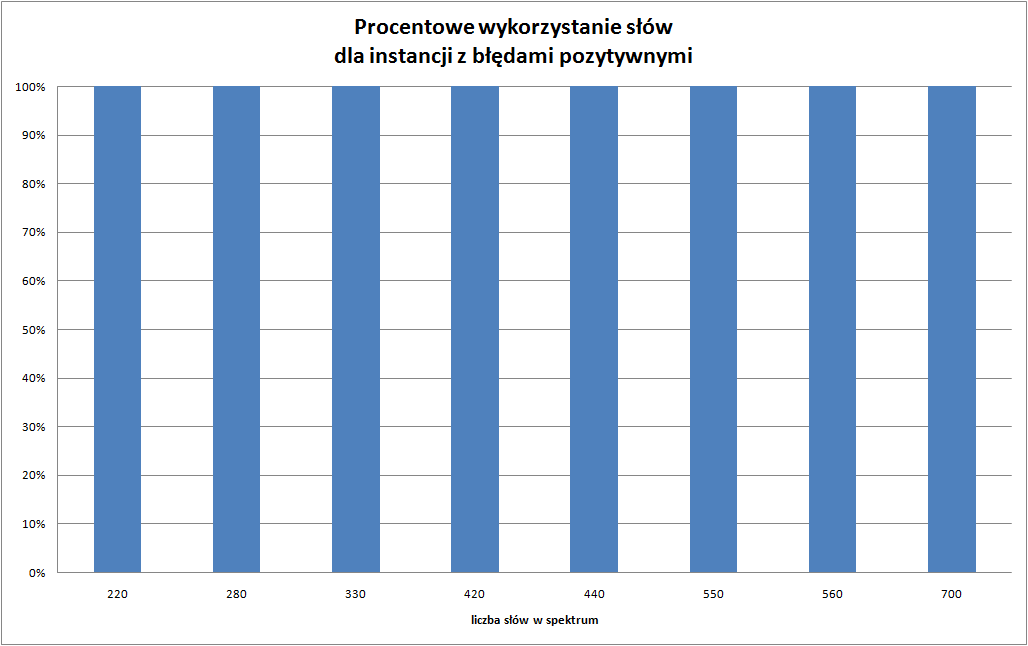
\includegraphics[width=\textwidth,keepaspectratio]{percentageUsedWords_general_positive.png}
 % \caption{}
\end{figure}

Jak widać na powyższym wykresie algorytm ten radzi sobie z błędami pozytywnymi bez problemów, dając za każdym razem wynik dokładny. Wynika to z charakterystyki tego typu instancji - zawsze można wyróżnić "główną ścieżkę" sekwencji, która musi stanowić po prostu rozwiązanie, a nasz algorytm takiej ścieżki właśnie szuka.

\begin{figure}[h]
  \footnotesize\centering
  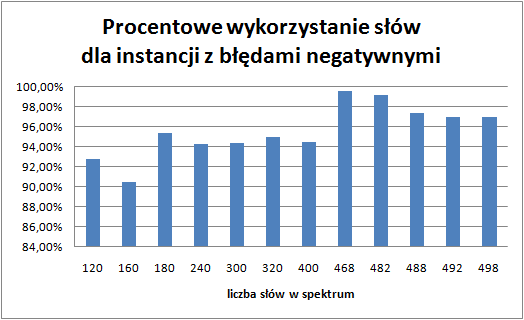
\includegraphics[width=\textwidth,keepaspectratio]{percentageUsedWords_general_negative.png}
 % \caption{}
\end{figure}

W przypadku instancji z błędami negatywnymi jest już nieco gorzej. W teorii wszystkie słowa wchodzące w skład spektrum powinny zostać wykorzystane. Nasz algorytm jest algorytmem zachłannym - skleja najkorzystniejsze w danej chwili dla niego sekwencji. Mając na uwadze to, że instancje składają się z prostych lasów grafowych, które w większości zawierają po prostu łańcuchy lub proste grafy, w pierwszym kroku następuje właśnie sklejenie tych łańcuchów. Gdyby nie ograniczenie na długość sekwencji wyjściowej, algorytm wykorzystywałby wszystkie słowa z instancji. Poniżej znajduje się wykres z długościami wyjściowych sekwencji jeśli pominiemy ograniczenie nałożone na długość sekwencji w zestawieniu z liczbą niewykorzystanych słów przez wersję algorytmu z tym ograniczeniem.

\begin{figure}[h]
  \footnotesize\centering
  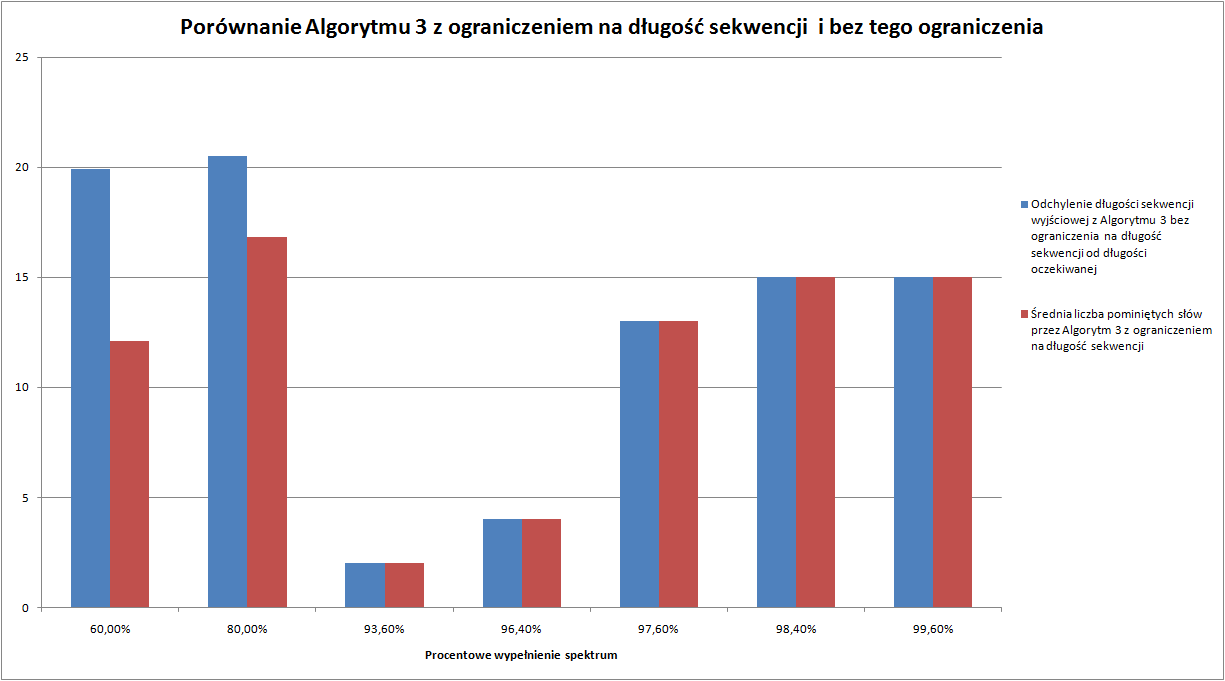
\includegraphics[width=\textwidth,keepaspectratio]{withoutNConstraint_general_negative.png}
 % \caption{}
\end{figure}

Wydaje się, że różnica jest dość uzasadniona - wersja algorytmu pilnująca długości sekwencji obcina po prostu w ostatnim kroku jedną z sekwencji o nadmiar znaków. Ten nadmiar znakowy przesunięty może być maksymalnie o 9 znaków (dla słów długości 10), więc ilość niewykorzystanych słów powinna być mniejsza o conajwyżej 9 względem odchylenia długości sekwencji od długości oczekiwanej w wersji algorytmu bez ograniczenia. I tak też się dzieje. Widać ponadto, że przy dużych wypełnieniach (ponad 90\%) spektrum ta różnica wynosi 0 - ostatnie "doklejenie" odbywa się po prostu na łukach o wartości równej licznie nadmiarowych znaków w przypadku gdybyśmy nie posiadali ograniczenia na długość sekwencji . Dla przykładu jeśli doklejamy $TACGT$ z przesunięciem dwa do $GCTA$, i odcinamy nadmiar znaków równy 2, to w efekcie mamy sekwencję $GCTAC$. Odcięliśmy dwa znaki, z których mielibyśmy słowa $ACG$ oraz $CGT$.

\begin{figure}[h]
  \footnotesize\centering
  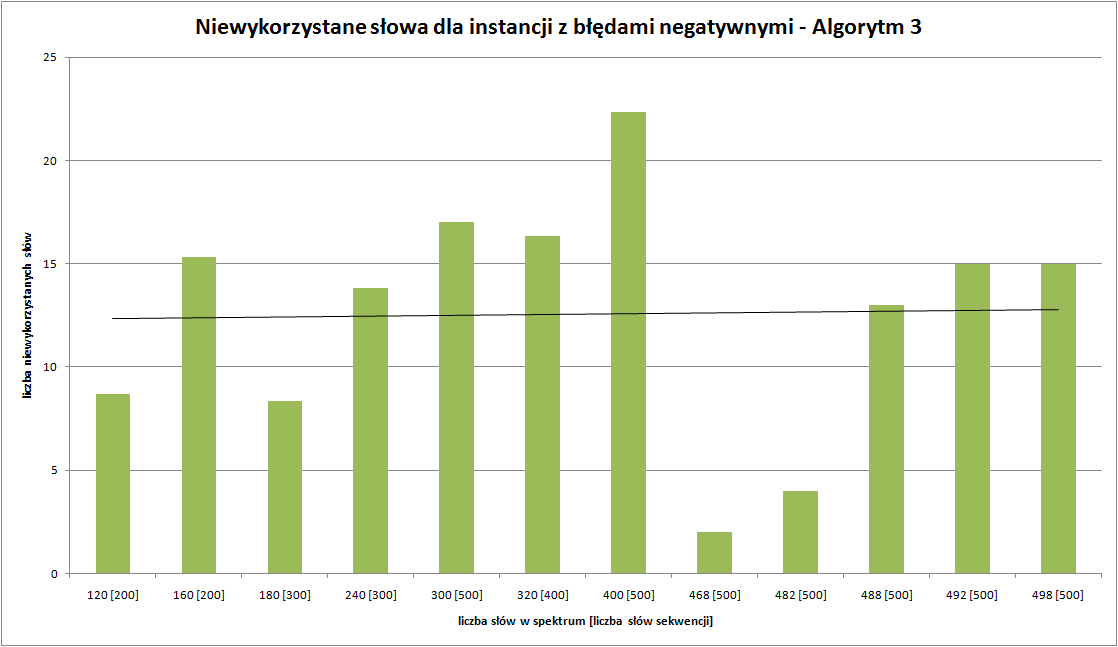
\includegraphics[width=\textwidth,keepaspectratio]{unusedWords_general_negative.png}
 % \caption{}
\end{figure}

Na wykresie obrazującym liczbę niewykorzystanych słów z instancji dla poszczególnych wielkości instancji widać, że nie są to duże braki. Zaznaczona na czarno linia trendu pokazuje, że średnio 12-13 słów jest niewykorzystanych, co daje dość dużą skuteczność algorytmu (ponad 90% jak wcześniej pokazano).

\subsection{Algorytm 2}

Algorytm specyficzny dla problemów z błędami pozytywnymi jest tak naprawdę szczególnym przypadkiem algorytmu ogólnego. Różnica polega na tym, że algorytm ten nie uwzględnia w ogóle łuków o kosztach wyższych niż jeden. Wynika to z obserwacji, że w instancji z błędami pozytywnymi (a więc z nadmiarem słów) musi istnieć ścieżka oparta o łuki o koszcie 1, która zawiera dokładnie $n$ wierzchołków. Algorytm ten poszukuje właśnie takiej ścieżki. Zauważmy, że wykres procentowego wykorzystania słów z instancji dla Algorytmu 2 wygląda identycznie jak analogiczny wykres dla Algorytmu 3. Jedynym sensownym porównaniem wydaje się być porównanie czasowe.

\subsection{Algorytm 4}

Algorytm specyficzny dla problemów z błędami negatywnymi jest zmodyfikowaną wersją algorytmu ogólnego. Różnią się one metodą wyznaczania wartości kosztów na łukach oraz rodzajem łuków najbardziej porządanych w rozwiązaniu (Algorytm 3 szuka najniższego kosztu, Algorytm 4 szuka najwyższego zysku). Mimo tak niewielkiej zmiany możemy zaobserwować na poniższym wykresie znaczny wzrost skuteczności algorytmu w wykorzystywaniu słów tworzących daną instancję.

\begin{figure}[h]
  \footnotesize\centering
  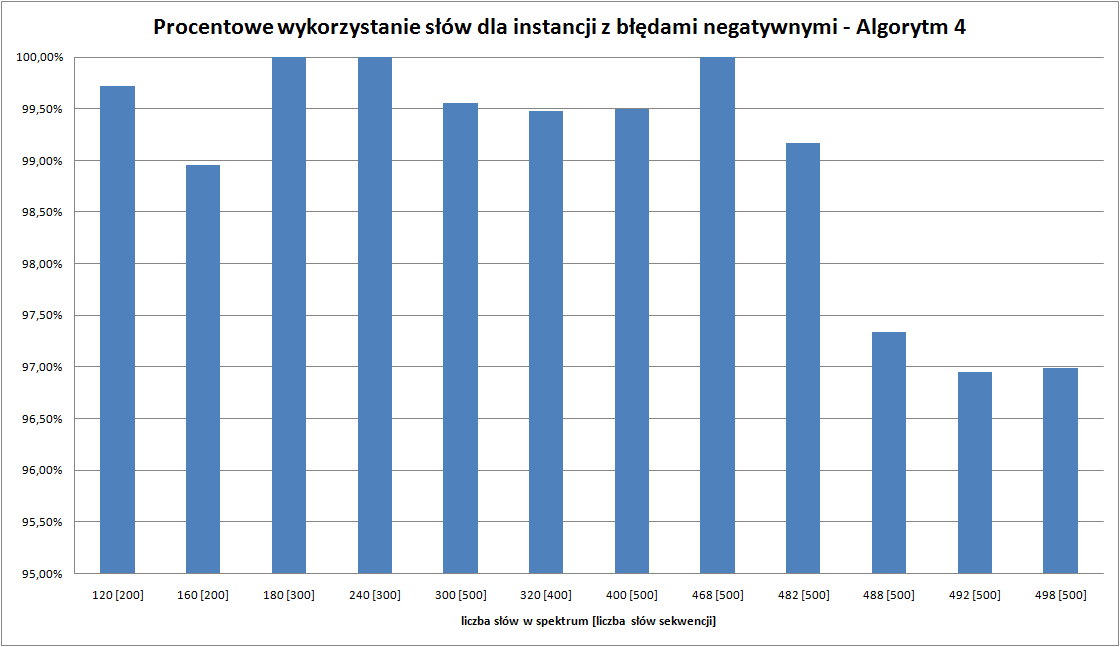
\includegraphics[width=\textwidth,keepaspectratio]{percentageUsedWords_negative.png}
 % \caption{}
\end{figure}

Siłą rzeczy algorytm ten popełnia mało błędów. Jako błąd traktuje się niewykorzystanie słowa z instancji. W większości przypadków pomijane są góra 2 słowa. Jedynie dla instancji niemalże bezbłędnych, w których brakuje mniej niż 10 słów algorytm ma mniejsze pole do popisu i zostawia większą liczbę słów.

\begin{figure}[h]
  \footnotesize\centering
  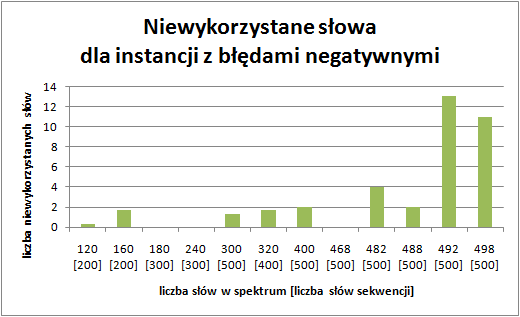
\includegraphics[width=\textwidth,keepaspectratio]{unusedWords_negative.png}
 % \caption{}
\end{figure}

\subsection{Algorytm 2 kontra Algorytm 3}

\begin{figure}[h]
  \footnotesize\centering
  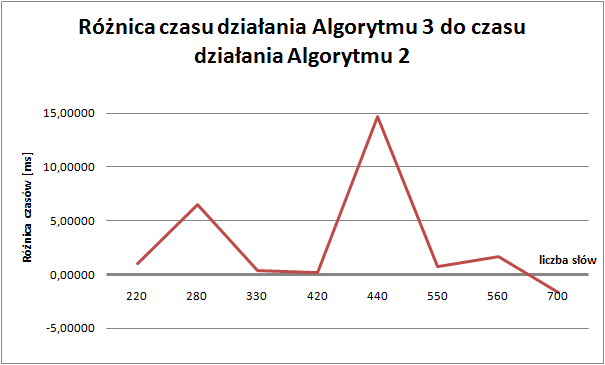
\includegraphics[width=\textwidth,keepaspectratio]{timeDiff_general_vs_positive.png}
 % \caption{}
\end{figure}

Jak widać na powyższym wykresie istnieje minimalna różnica czasowa w działaniu tych dwóch algorytmów. Przypadek okrojony działa o tysięczne sekundy szybciej, ponieważ nie ma narzutu na sprawdzanie warunku stopu oraz nie są tworzone kilkukrotnie sekwencję z dotychczasowych rozwiązań. Jednak w związku z tak niewielkimi różnicami można powiedzieć, że algorytmy te są porównywalne dla zbioru instancji z błędami pozytywnymi.
Gdybyśmy uruchomili algorytm dla instancji z błędami negatywnymi otrzymalibyśmy mierny wynik, ponieważ zostałby uwzględniony tylko jeden graf wchodzący w skład lasu grafów który jest badaną instancją.

\subsection{Algorytm 4 kontra Algorytm 3}

\begin{figure}[h]
  \footnotesize\centering
  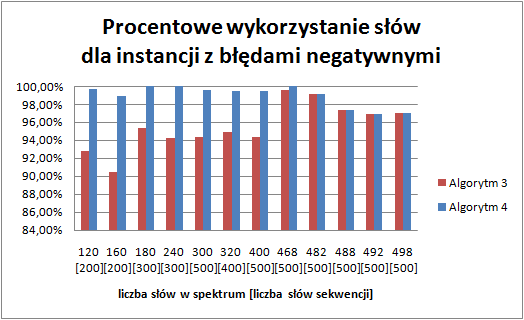
\includegraphics[width=\textwidth,keepaspectratio]{percentageUsedWords_general_vs_negative.png}
 % \caption{}
\end{figure}

Porównując z kolei algorytm dla błędów negatywnych względem algorytmu ogólnego od razu widzimy, że ten pierwszy jest lepszy - wykorzystuje bowiem średnio $98,97\%$ słów zadanej instancji! Jednak można zauważyć, że choć tak niewielka różnica w działaniu algorytmu ma wpływ dla instancji z dużą ilością brakujących słów, o tyle dla instancji w których brakuje mniej niż 20 słów wyniki są identyczne. Wynika to z tego, że główny "silnik" sklejania sekwencji jest w zasadzie identyczny, tj szuka najdłuższego możliwego łańcucha oligonukleotydów.

\end{document}
